%% PhyNetPy 1.0.0 software paper
%%
%% Target venue: Oxford Bioinformatics (Applications Note / Original Paper).
%% The journal supplies its own class at submission; this file uses the
%% standard `article' class so that it compiles anywhere, including a bare
%% Overleaf project. Switching to the journal class should require changing
%% only the \documentclass line and the title block.
%%
%% Numeric tables and the performance figure are generated by
%% benchmarks/make_artifacts.py from the benchmark JSON. Do not edit
%% tables/*.tex by hand.

\documentclass[11pt]{article}

\usepackage[T1]{fontenc}
\usepackage[utf8]{inputenc}
\usepackage[margin=1in]{geometry}
\usepackage{graphicx}
\usepackage{array}      % >{...} column specifiers used by tables/analyses.tex
\usepackage{booktabs}
\usepackage{amsmath}
\usepackage{amssymb}
\usepackage{listings}
\usepackage{xcolor}
\usepackage{tikz}
\usetikzlibrary{arrows.meta,positioning,fit,backgrounds}
\usepackage[numbers,sort&compress]{natbib}
\usepackage[hidelinks]{hyperref}
\usepackage{microtype}

\graphicspath{{figures/}}

% ---------------------------------------------------------------------------
% Code listings
% ---------------------------------------------------------------------------
\definecolor{codekeyword}{RGB}{0,92,197}
\definecolor{codestring}{RGB}{3,106,64}
\definecolor{codecomment}{RGB}{106,115,125}

\lstdefinestyle{python}{
  language=Python,
  basicstyle=\ttfamily\small,
  keywordstyle=\color{codekeyword},
  stringstyle=\color{codestring},
  commentstyle=\itshape\color{codecomment},
  showstringspaces=false,
  breaklines=true,
  frame=single,
  rulecolor=\color{codecomment},
  framesep=4pt,
  xleftmargin=6pt,
  columns=fullflexible,
  keepspaces=true,
  literate={-}{-}1 {_}{{\_}}1,
}
\lstset{style=python}

\newcommand{\phynetpy}{\textsc{PhyNetPy}}
\newcommand{\phylonet}{\textsc{PhyloNet}}
% Identifiers are written with literal underscores, as they appear in the
% source. \detokenize makes them printable in text mode, so \code{infer_network}
% needs no escaping and cannot silently become a subscript.
\newcommand{\code}[1]{\texttt{\detokenize{#1}}}

% ---------------------------------------------------------------------------
\title{\phynetpy: a Python framework for phylogenetic network analysis
and inference}

\author{%
  Mark Kessler\thanks{Corresponding author: \texttt{mak17@rice.edu}}
  \and Luay Nakhleh%
}
\date{Department of Computer Science, Rice University}

\begin{document}
\maketitle

\begin{abstract}
\noindent
\textbf{Motivation.} Phylogenetic network methods have accumulated faster than
the software infrastructure to support them. PhyloNet established a body of
network-analysis methods and the computational ecosystem around them, and much
of the field's methodological work now assumes that body of methods exists. New
methods, however, are typically built as standalone programs, each supplying its
own network representation, search machinery and input handling, and most are not
reachable from the Python environment where comparative and statistical analysis
is now usually done.

\noindent
\textbf{Results.} We present \phynetpy, a Python library for phylogenetic network
inference and analysis. Inference is expressed as two verbs, \code{infer} and
\code{score}, parameterised on three independent axes: the data observed, the
generative model, and the statistical criterion. A method is a cell in that
product rather than a command name, and dispatch runs through a registry that
doubles as a machine-readable statement of which combinations are defined,
which are unimplemented, and which are meaningless. Version 1.0.0 provides seven
inference methods, six of them reimplementations of published PhyloNet analyses;
a reusable rooted-DAG network type with ploidy and typed branch-length units;
nine network dissimilarity measures and a separate reticulation-specific
comparison module; coalescent, sequence and biallelic-marker simulation; and
MCMC convergence diagnostics with Tracer-compatible output. The library holds
1{,}130 tests, and a harness cross-validates its multispecies-network-coalescent
density and Felsenstein likelihood against PhyloNet's own implementations across
14 adversarial cases, agreeing to $10^{-5}$. On matched pseudo-likelihood
inference from identical gene trees, \phynetpy\ runs faster than PhyloNet by a
margin that grows with dataset size, but recovers the generating topology about
half as often across 30 trials; we report that discrepancy and the diagnostic
work it still needs rather than a net verdict.

\noindent
\textbf{Availability.} \code{pip install phynetpy}. Source, documentation and the
scripts reproducing every figure and table here are at
\url{https://github.com/NakhlehLab/PhyNetPy}, under the MIT license.
\end{abstract}


\section{Introduction}
\label{sec:introduction}

Species histories are not always trees. Hybridization, introgression and
allopolyploidy move genetic material between diverging lineages, and the result
is a reticulate history that a tree cannot express
\cite{TODO_networks_review}. Inferring such histories is harder than inferring
trees for two reasons that compound: the space of networks is larger and less
well behaved than the space of trees, and the same gene-tree discordance that
hybridization produces is also produced by incomplete lineage sorting
\cite{TODO_ILS_review}. Distinguishing the two requires a model in which both
occur, which is what the multispecies network coalescent provides
\cite{TODO_MSNC}.

Over roughly fifteen years PhyloNet \cite{Than2008PhyloNet,
Wen2018InferringPhyloNet} assembled the methods this implies: parsimony,
maximum likelihood, pseudo-likelihood, and Bayesian inference, from gene trees,
from sequence alignments, and from biallelic markers, with extensions to
polyploid complexes. Its importance to the field is not in dispute and this
paper does not argue otherwise. A researcher today who wants to infer a
phylogenetic network from gene trees reaches for PhyloNet, and should.

What has changed is the surrounding computational environment. Three specific
frictions motivated this work.

First, a PhyloNet analysis is specified in a NEXUS file containing a command
block and run through the JVM. That design is well suited to running an analysis
and poorly suited to embedding one: a sweep over conditions means generating
files, and consuming the result means parsing text. Comparative and statistical
analysis in phylogenetics now largely happens in Python, alongside NumPy
\cite{Harris2020NumPy} and SciPy \cite{Virtanen2020SciPy}, and the tree-oriented
libraries that serve that environment -- DendroPy \cite{Sukumaran2010DendroPy},
ETE \cite{HuertaCepas2016ETE3}, Biopython \cite{Cock2009Biopython} -- have no
network counterpart.

Second, a method developer starting a new network method starts from very little.
A network representation, traversal and cluster machinery, topology moves, a
search driver, parameter optimisation, input parsing and convergence diagnostics
are all prerequisites to testing a new scoring criterion, and none of them are
what the new method is about. The predictable outcome is that each new method
ships as a separate program with its own representation, and that comparing two
methods means reconciling two file formats.

Third, the organisation of a method set as a list of command names hides its
structure. Most of those commands vary along the same three dimensions -- the
data, the assumed generative process, the optimality criterion -- and a list
does not say which combinations exist, which are unimplemented, and which are
not meaningful at all. A user cannot tell the difference between a feature that
is missing and a request that does not make sense.

\phynetpy\ addresses these. It is a Python library in which the network is a
reusable data structure, inference is two verbs over three typed axes, and the
set of available methods is queryable at runtime. Its inference methods are, for
the most part, reimplementations of PhyloNet's, which is deliberate: the point is
not new statistics but a foundation on which new statistics can be built and
against which existing results can be checked.

\paragraph{Contributions.}
\begin{itemize}
  \item A network representation and analysis layer usable independently of any
    inference method: a rooted DAG with ploidy, typed branch-length units, nine
    dissimilarity measures, blob and cluster decomposition, and MUL-tree
    conversion (Sections~\ref{sec:architecture} and~\ref{sec:functionality}).
  \item An inference interface of two verbs over the product of data, model and
    criterion, with dispatch through a registry that distinguishes undefined,
    unimplemented and ill-typed requests, and that serves as the extension point
    for contributed methods (Section~\ref{sec:architecture}).
  \item Seven implemented inference methods, six corresponding to published
    PhyloNet analyses, with the gaps relative to PhyloNet stated explicitly
    (Section~\ref{sec:functionality}).
  \item Numerical cross-validation against PhyloNet's own implementations of the
    multispecies-network-coalescent density and the Felsenstein likelihood,
    across 14 adversarial cases (Section~\ref{sec:validation}).
  \item A replicated head-to-head runtime and accuracy comparison on identical
    input, reporting a runtime advantage and an accuracy deficit, with the
    accuracy result left open rather than explained away
    (Section~\ref{sec:validation}).
  \item A migration account for existing PhyloNet users, including what does not
    carry over (Section~\ref{sec:comparison}).
\end{itemize}

\section{Background}
\label{sec:background}

This section fixes terminology and names the four criterion families the library
implements. Readers familiar with network inference can skip to
Section~\ref{sec:architecture}.

\subsection{Networks}

A rooted phylogenetic network is a rooted directed acyclic graph whose leaves are
labelled by sampled taxa. Nodes of in-degree one are tree nodes and represent
ordinary divergence; nodes of in-degree two or more are reticulation nodes and
represent an event in which a lineage derives material from more than one parent.
Edges entering a reticulation carry inheritance probabilities $\gamma$ summing to
one, giving the proportion of loci descending through each parent.

A network with no reticulation nodes is a tree, which is why \phynetpy\ does not
give trees a separate type. Two derived notions recur. A \emph{displayed tree} is
obtained by retaining one incoming edge at each reticulation and suppressing the
rest; a network on $r$ reticulations displays up to $2^r$ trees, each with a
probability given by the product of the retained $\gamma$ values. A \emph{blob}
is a biconnected component, and contracting each blob to a node yields the
\emph{tree of blobs}, which captures the part of the history that is unambiguously
tree-like. Network \emph{level} is the largest number of reticulations in any
single blob, and bounds how entangled the reticulate structure is.

Branch lengths are measured on more than one scale. Sequence-based methods work
in expected substitutions per site; coalescent methods work in coalescent units,
related through the population-size parameter $\theta = 4N\mu$. The two are not
interchangeable, and a network carrying lengths on one scale will produce
plausible but wrong answers if read on the other.

\subsection{Criteria}

\paragraph{Parsimony.} Minimising deep coalescences (MDC) counts the extra
lineages implied by embedding observed gene trees in a candidate species history
and prefers the history requiring fewest \cite{Than2009MDC}. It needs only
gene-tree topologies, is cheap, and assumes no probabilistic model. Under
polyploidy the criterion is applied to a multiply-labelled tree, in which a
polyploid taxon appears once per subgenome \cite{Yan2022Allop}.

\paragraph{Likelihood.} Under the multispecies network coalescent, the
probability of a gene tree given a network is obtained by summing over the ways
lineages can be routed through reticulations and coalesce within branches
\cite{Yu2014ML}. This uses all the information in the data and is the most
expensive of the criteria, since the sum grows quickly with taxa and
reticulations.

\paragraph{Pseudo-likelihood.} Replacing the full likelihood with a product over
subsets of taxa -- in practice rooted triplets -- yields a composite objective
that is far cheaper and retains enough signal to rank topologies
\cite{Yu2015MPL}. The cost is that the product is not a normalised probability of
the data, which is why it cannot serve as a posterior target.

\paragraph{Bayesian inference.} Sampling networks from a posterior requires
proposals that change dimension, since adding or removing a reticulation changes
the parameter count; reversible-jump MCMC supplies the machinery
\cite{Green1995RJMCMC, Hastings1970}. Samplers exist for gene trees as data, for
sequence alignments with gene trees treated as latent variables
\cite{Wen2018MCMCSEQ}, and for biallelic markers, where the marker likelihood is
computed exactly without gene trees \cite{Bryant2012SNAPP, Zhu2018BiMarkers}.

The grouping above is the reason \phynetpy's interface has the shape it does.
Across these four families the data type, the assumed generative process and the
objective vary independently, so the natural parameterisation of the method set
is a product of three axes rather than a list of names.

\section{Software architecture}
\label{sec:architecture}

Figure~\ref{fig:architecture} shows how \phynetpy\ is put together. The
organising decision is that no analysis owns the network. A network is a data
structure that the library provides; scoring criteria, generative models,
topology moves and search drivers are separate things that act on it. Almost
everything else in this section follows from that separation.

\begin{figure}[t]
  \centering
  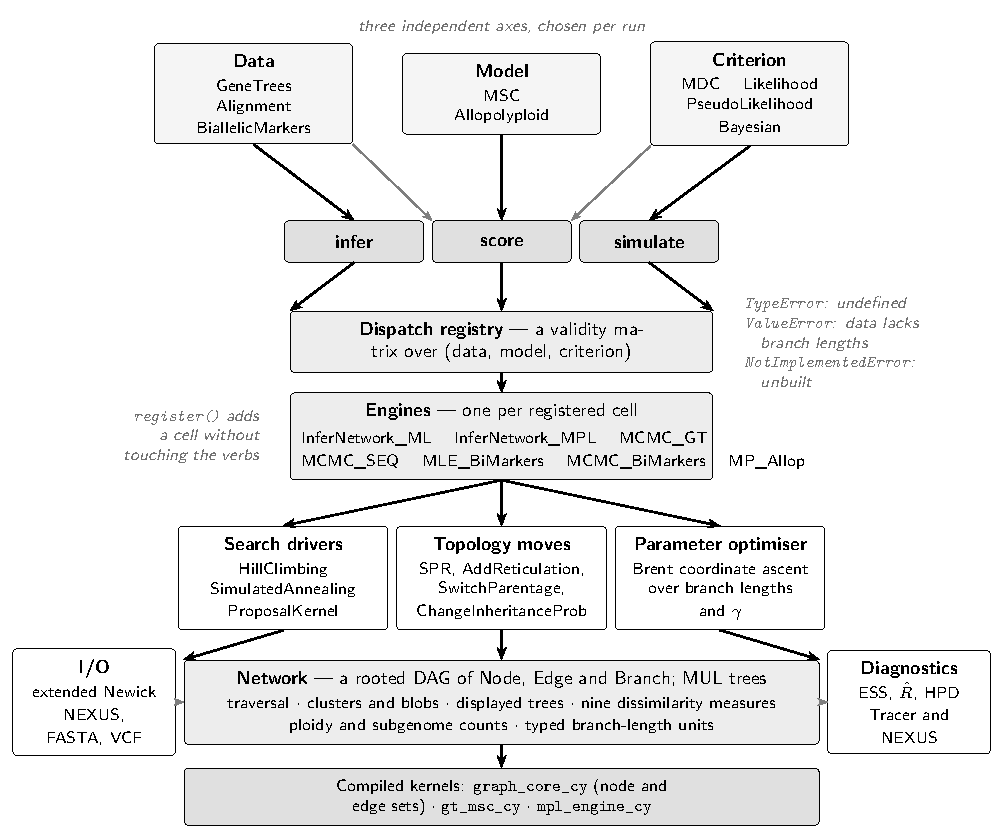
\includegraphics[width=\linewidth]{architecture.pdf}
  \caption{\phynetpy\ organised by dependency. A run is specified by picking
  one object from each of the three axes at the top and calling one of the
  three verbs. The registry resolves that triple to an engine. Engines do not
  implement their own search machinery, topology moves, parameter optimisation
  or network operations; they compose the shared components below them. The
  compiled kernels sit under the network layer and are not part of the public
  interface.}
  \label{fig:architecture}
\end{figure}

\subsection{The network as a reusable object}

\code{Network} is a rooted directed acyclic graph over \code{Node} and
\code{Edge}, with \code{Branch} carrying length, inheritance probability and
tag. Trees are not a separate type: a tree is a network with no reticulation
nodes, and the same code paths serve both. Gene trees supplied as input are
\code{Network} instances, which is why a gene tree and an inferred species
network can be passed to the same distance function.

Reticulation in-degree is not capped at two. \code{Network.get_parents}
imposes no limit and \code{add_edges} does not check parent counts, so a node
representing an unresolved or aggregated reticulation with three or more
parents is representable. Some analyses do assume the binary case --
\code{reticulation_tripartitions} requires exactly two parents, for instance --
so the generality lives in the representation rather than throughout the
library.

The operations on \code{Network} are the ones network methods keep needing:
topological ordering, breadth- and depth-first traversal, most recent common
ancestors, leaf-descendant sets for all nodes at once, induced subnetworks,
acyclicity checking, and copying. Ploidy is first class through
\code{subgenome_count} and the corresponding edge queries, and conversion to a
multiply-labelled (MUL) tree is implemented because the allopolyploid parsimony
criterion is defined on that representation.

Two design choices in this layer are worth stating because they change what
callers can get wrong. Branch lengths carry an explicit unit --
\code{SUBSTITUTIONS_PER_SITE}, \code{COALESCENT_2N}, or
\code{UNSPECIFIED} -- and \code{convert_network_branch_lengths} refuses to
convert when either side is unspecified rather than guessing. Coalescent
methods and sequence methods read branch lengths on different scales, and
mixing them produces plausible numbers rather than an error, so the unit is
tracked on the network instead of being left to the user's discipline. Second,
the node and edge containers are compiled (\code{graph_core_cy}) and maintain
indices for incidence and name lookup, because network search evaluates large
numbers of candidate topologies and the cost of a single edge insertion sets
the ceiling on tractable problem size.

\subsection{Three axes and three verbs}

A phylogenetic network method is usually presented as a named procedure. Seen
from the software side, most of those names vary along three independent
dimensions: the data observed, the generative process assumed, and the
statistical objective optimised. \phynetpy\ makes those three dimensions
explicit arguments and reduces the interface to three verbs.

\code{infer} searches for a network. \code{score} evaluates one. \code{simulate}
runs the axes backwards, taking a model and a network and returning a data
object. The axes are:

\begin{itemize}
  \item \textbf{Data} --- \code{GeneTrees}, \code{Alignment},
    \code{BiallelicMarkers}. Each carries the species-to-allele mapping, and
    each knows its own type, so a caller never declares what kind of data it
    is passing.
  \item \textbf{Model} --- \code{MSC}, the multispecies network coalescent with
    a population parameter $\theta = 4N\mu$, and \code{Allopolyploid}, which
    takes a subgenome map. The generative process used to be implicit in which
    scorer a user selected.
  \item \textbf{Criterion} --- \code{MDC} (minimising deep coalescences),
    \code{Likelihood}, \code{PseudoLikelihood}, and \code{Bayesian}.
\end{itemize}

\code{Bayesian} wraps an objective rather than sitting beside the likelihoods:
\code{Bayesian(objective=Likelihood())}. Sampling a posterior is a mode of
working with a likelihood, not a fourth thing to optimise, and expressing it
that way means \code{Bayesian} inherits the data types its objective accepts
instead of restating them.

The practical consequence is that changing method means changing an argument.
The same call that maximises a pseudo-likelihood samples a posterior if the
criterion changes, and \code{infer} returns the same type either way:
\code{InferenceResult} carries \code{.best}, \code{.score}, \code{.trace}, and
\code{.posterior}, the last populated only for Bayesian runs. Attribute access
falls through to \code{.raw}, the engine's native result, so per-method
richness -- log writers, information criteria, reticulation posteriors --
remains reachable without the wrapper having to enumerate it.

\subsection{Dispatch as a validity matrix}

Whether a run makes sense depends on the whole triple, not on any one axis. A
parsimony criterion over a sequence alignment is not a missing feature; it is a
category error, since minimising deep coalescences is defined over gene-tree
topologies. Maximum parsimony from gene trees under the \code{MSC}, by
contrast, is perfectly well defined and simply has no implementation here yet.
A criterion that needs branch lengths applied to gene trees that lack them is a
third, different problem.

\code{resolve} in \code{_registry.py} separates these three cases and raises
accordingly: \code{TypeError} when the criterion is not defined on that data
type, \code{ValueError} when the data lack branch lengths the criterion
requires, and \code{NotImplementedError} when the combination is meaningful but
unbuilt. Conflating them is what makes an unsupported request hard to act on:
a user cannot tell whether to supply different data, wait for a release, or
abandon the idea.

Because dispatch is a registry keyed on the triple, the set of available
methods is introspectable. \code{validity_matrix()} tabulates it, and the table
is built from the registry rather than maintained alongside it, so it cannot
fall out of date. \code{registered_cells()} lists every implemented
combination; Table~\ref{tab:analyses} is generated from that call.

\subsection{Extension}

Adding a method means registering a cell:

\begin{lstlisting}
@register(GeneTrees, MSC, MyCriterion)
class MyEngine(Engine):
    method = "MyMethod"

    def infer(self, data): ...
    def score(self, network, data, optimize=False): ...
\end{lstlisting}

What an engine author does not write is the rest of the run. The search drivers
(\code{HillClimbing}, \code{SimulatedAnnealing}, and the \code{ProposalKernel}
interface), the ten topology-move classes, the Brent coordinate-ascent
optimiser for branch lengths and inheritance probabilities, the I/O layer and
the chain diagnostics are shared. This is the claim in the paper's title that
rests on design rather than measurement, so it is worth being precise about the
evidence: the registry is exercised by all seven of the library's own methods,
which is a weaker statement than demonstrating that an outside contributor
found it sufficient.

One cross-cutting option illustrates the difference between a constraint and a
hint. A starting phylogeny can be supplied as \code{Start(net)}, a free
starting point, or as \code{Start(net, StartMode.AUGMENT)}, which requires the
result to contain that network. The second is enforced by a cluster-containment
check in the accept path rather than approximated by withholding moves, which
is possible because adding reticulations to a network preserves its clusters.
Engines whose proposal kernels cannot honour it -- \code{MCMC_SEQ} and the
allopolyploid search -- reject the request explicitly instead of accepting it
and quietly doing something else.

\subsection{Compiled kernels}

Four Cython modules are compiled at install time. \code{graph_core_cy} provides
the node and edge containers; \code{gt_msc_cy} and \code{mpl_engine_cy}
accelerate the gene-tree coalescent likelihood and the pseudo-likelihood
dynamic program. The fourth, \code{seq_engine_cy}, is compiled but not yet
called from \code{_seq_likelihood.py}.

None of these are part of the public interface, and the graph core is a hard
requirement rather than an optional accelerator: \code{Network} imports it at
module load and raises with build instructions if it is absent. That removes a
class of bug in which a user unknowingly runs a slower parallel implementation,
at the cost of requiring a C compiler when installing from source.
Section~\ref{sec:validation} reports what the compiled pseudo-likelihood kernel
is worth against the pure-Python path that remains in the repository as a
reference.

\section{What version 1.0.0 does}
\label{sec:functionality}

\subsection{Inference}

Table~\ref{tab:analyses} lists the analyses available, generated from
\code{registered_cells()} so that it matches the release it describes. Seven
cells are implemented. Six correspond to PhyloNet commands and are
reimplementations of published methods; the seventh, maximum-parsimony
inference under polyploidy, is a new implementation of the method PhyloNet
exposes as \code{InferNetwork_MP_Allopp} and differs from it in its proposal
kernel.

\begin{table}[t]
  \centering
  \scriptsize
  % Generated by benchmarks/make_analyses_table.py from phynetpy.infer.registered_cells().
% Do not edit by hand.
\setlength{\tabcolsep}{3pt}
\begin{tabular}{@{}l>{\raggedright\arraybackslash}p{15mm}>{\raggedright\arraybackslash}p{18mm}>{\raggedright\arraybackslash}p{16mm}>{\raggedright\arraybackslash}p{37mm}l>{\raggedright\arraybackslash}p{17mm}@{}}
\toprule
Engine & Data & Model & Criterion & Problem addressed & PhyloNet command & Status \\
\midrule
\texttt{MCMC\_GT} & Gene trees & MSC & Bayesian & Posterior over networks given gene trees \cite{Wen2016MCMCGT} & \texttt{MCMC\_GT} & Reimpl. \\
\texttt{InferNetwork\_ML} & Gene trees & MSC & Likelihood & Network topology and parameters by maximum likelihood \cite{Yu2014ML} & \texttt{InferNetwork\_ML} & Reimpl. \\
\texttt{InferNetwork\_MPL} & Gene trees & MSC & Pseudo-lik. & Network topology from gene-tree triplet frequencies \cite{Yu2015MPL} & \texttt{InferNetwork\_MPL} & Reimpl. \\
\texttt{MCMC\_SEQ} & Alignment & MSC & Bayesian & Joint posterior over networks and gene trees from sequences \cite{Wen2018MCMCSEQ} & \texttt{MCMC\_SEQ} & Reimpl. \\
\texttt{MCMC\_BiMarkers} & Markers & MSC & Bayesian & Posterior over networks from biallelic markers \cite{Zhu2018BiMarkers} & \texttt{MCMC\_BiMarkers} & Reimpl. \\
\texttt{MLE\_BiMarkers} & Markers & MSC & Likelihood & Exact marker likelihood of a given network \cite{Bryant2012SNAPP,Zhu2018BiMarkers} & \texttt{MLE\_BiMarkers} & Reimpl., scoring only \\
\texttt{MP\_Allop} & Gene trees & Allopolyploid & Parsimony & Parsimonious network under polyploidy, minimising deep coalescences \cite{Yan2022Allop,Than2009MDC} & \texttt{InferNetwork\_MP\_Allopp} & New impl. \\
\midrule
\multicolumn{7}{@{}l}{\emph{Cells that are well defined but carry no engine}} \\
--- & Gene trees & MSC & Parsimony & \emph{raises} \texttt{NotImplementedError} & \texttt{InferNetwork\_MP} & Sched. 1.0.0 \\
--- & Markers & MSC & Pseudo-lik. & \emph{raises} \texttt{NotImplementedError} & \texttt{MLE\_BiMarkers -pseudo} & Sched. 1.0.0 \\
--- & Alignment & MSC & Likelihood & \emph{raises} \texttt{NotImplementedError} & \texttt{---} & Not planned \\
\bottomrule
\end{tabular}

  \caption{Analyses in \phynetpy\ 1.0.0. Rows are generated from the dispatch
  registry. ``Reimplementation'' means the method was published elsewhere and
  implemented here from its description; the \code{MP_Allop} row is marked as
  a new implementation because its search uses a single ploidy-preserving move
  rather than the six moves of the original. The lower block lists
  combinations that are well defined but carry no engine, and therefore raise
  \code{NotImplementedError} rather than failing obscurely.%
  }
  \label{tab:analyses}
\end{table}

Three points about that table matter more than its length.

The first is what is \emph{not} in it. Maximum parsimony from gene trees under
diploid hybridization -- PhyloNet's \code{InferNetwork_MP} -- is a legal cell
with no engine behind it. The only parsimony code in \phynetpy\ is defined on
multiply-labelled trees for the allopolyploid model, so the diploid case is
genuinely absent rather than partially present. The biallelic
pseudo-likelihood is absent for the same kind of reason: the marker code
computes the full likelihood only. Both are scheduled for
1.0.0.\footnote{[TODO: verify at 1.0.0. At the time of writing these two cells
raise \code{NotImplementedError}; the manuscript must be updated with measured
behaviour once they are built, or this claim removed.]}

The second is a limitation inside a row that is otherwise marked available.
\code{MLE_BiMarkers} can score a given network but cannot search: its
\code{infer} path raises unconditionally. A reader comparing feature lists
would otherwise reasonably assume that maximum-likelihood network inference
from markers is available.

The third concerns \code{Bayesian(objective=PseudoLikelihood())}, which is
refused. A triplet pseudo-likelihood is not a normalised probability of the
data, so using it as a Metropolis--Hastings target does not yield a calibrated
posterior. The combination is mechanically easy to allow and would produce
numbers; it is rejected because those numbers would not mean what a reader of
the output would take them to mean.

Search behaviour is controlled by presets rather than by combinations of
booleans. Four are provided: \code{default}, \code{fast}, \code{accurate}, and
\code{phylonet}. The last exists to reproduce PhyloNet's
optimise-everything-per-topology behaviour, which is what makes cross-checking
against it meaningful; individual flags override the preset.

\subsection{Network analysis}

The analysis layer is usable without running any inference, and is where a
researcher comparing methods or summarising results spends time.

Nine dissimilarity measures are implemented: the $\mu$ (path-multiplicity)
distance \cite{Cardona2009MuDistance}, hardwired and softwired cluster
distances, Robinson--Foulds over hardwired clusters, tripartition distance,
displayed-tree distance, average and weighted average path distance
\cite{TODO_APD}, and a pairwise leaf distance; \code{Network} additionally
provides a rooted triplet distance. The cluster, tripartition and
displayed-tree measures accept a \code{normalize} argument returning a value in
$[0,1]$.

A separate module compares networks by the reticulations they assert rather
than by overall topology, through reticulation tripartitions, a dissimilarity
built on them, and precision and recall against a reference network. Whether an
inferred network recovers the \emph{right hybridizations} is the question a
biologist usually has, and a whole-network distance answers it only indirectly.

Decomposition covers displayed trees with their probabilities, the dominant
tree, hardwired and softwired clusters, biconnected components (blobs) and the
tree of blobs, network level, bridges and articulation points, and induced
subnetworks by taxon set.

\subsection{Simulation}

\code{simulate} is the generative inverse of \code{infer} and returns a
data-axis object, so a recovery check is two calls with nothing in between:

\begin{lstlisting}
sim = simulate(MSC(theta=0.02), taxa=6, n=200)
recovered = infer(sim, criterion=PseudoLikelihood())
\end{lstlisting}

Gene genealogies are simulated backwards in time within network branches under
the multispecies network coalescent, with lineages routed at reticulations
according to inheritance probabilities. Sequence evolution runs a continuous-time
Markov chain down each gene tree under JC69, HKY85 or GTR, single- or
multi-locus. Biallelic markers are simulated site by site, sampling an
independent genealogy per site. Species trees come from Yule or constant-rate
birth--death processes; networks are produced by drawing a tree and grafting
reticulations onto it.

Two limits are worth stating. Simulation under \code{Allopolyploid} raises
\code{NotImplementedError} -- only \code{MSC} has simulators. And because
reticulations are grafted onto a separately drawn tree, the network simulator
is not a birth--death--hybridization process in which hybridization and
speciation occur jointly, so it should not be used to study the distribution of
network shapes such a process induces.

One asymmetry catches users. The simulators write branch lengths in expected
substitutions per site while the gene-tree criteria read coalescent units, so a
round trip recovers the topology but not the lengths. The branch-length unit
tags described in Section~\ref{sec:architecture} make this visible rather than
silent.

\subsection{Data, I/O, and diagnostics}

Extended Newick, NEXUS, FASTA and VCF are supported for both reading and
writing. The extended Newick reader detects dialects and converts between them,
which matters because no single interchange convention is universal across
network software. PHYLIP is not supported.

Four alphabets are built in (DNA, RNA, protein, codon). Eight nucleotide
substitution models are provided -- JC, K80, F81, HKY, TN93, K81, SYM, GTR --
each parameterised by the free parameters its literature defines rather than by
a full exchangeability vector.

For posterior analysis, \phynetpy\ computes effective sample size,
autocorrelation time, standard error of the mean, highest-posterior-density
intervals, the Geweke statistic \cite{Geweke1992}, and the Gelman--Rubin
$\hat{R}$ across chains \cite{GelmanRubin1992}. Traces are written in Tracer
log format \cite{Rambaut2018Tracer} and tree samples in NEXUS, and Tracer logs
can be read back, so existing tooling applies to \phynetpy\ output without
conversion scripts. \code{reticulation_sweep} fits a range of reticulation
counts and reports information criteria, which addresses the standing problem
that a more reticulate network almost always fits the data better.

\section{Validation and performance}
\label{sec:validation}

Two questions are often run together and answered with the same number. Does
\phynetpy\ compute what it claims to compute? And how fast is it? The first is
a correctness question with a right answer; the second is a measurement that
depends on hardware, data, and what each implementation was asked to do. This
section keeps them apart.

All measurements below were taken on the platform recorded in
Section~\ref{sec:reproducibility} and are regenerated by scripts in the
repository; no figure in this section was entered by hand.

\subsection{Agreement with PhyloNet}

The strongest correctness evidence available for a reimplementation is
numerical agreement with the implementation it reimplements, on inputs chosen
to be difficult. \phynetpy\ ships a harness that compiles a Java driver
invoking PhyloNet's own classes -- \code{GeneTreeBrSpeciesNetDistribution} for
the multispecies-network-coalescent density, and its BEAGLE-backed
\cite{Ayres2012BEAGLE} \code{UltrametricTree} for the Felsenstein likelihood --
and feeds both implementations from one shared specification file, so a
disagreement is a real discrepancy rather than a difference in test setup.

Fourteen cases are specified, chosen to probe the places where two
implementations of the same density diverge: multiple alleles per species, GTR
with skewed base frequencies and asymmetric exchange rates, stacked
reticulations, boundary population sizes, embeddings of probability zero (where
both sides must agree on $-\infty$), IUPAC ambiguity codes and gaps,
branch-length saturation, fully constant alignments, and a five-taxon
caterpillar. The two quantities compared are
$\log P(g \mid \Psi)$ and $\log P(S \mid g)$.

All cases agree to within $10^{-5}$, and the $-\infty$ case matches exactly. The
suite runs as 23 pytest cases and skips cleanly when no PhyloNet jar or BEAGLE
installation is present, so it does not burden contributors who have neither.

This is a statement about two likelihood functions, not about two searches.
Agreement on a fixed network says nothing about whether the two searches visit
the same topologies, and Section~\ref{sec:headtohead} shows that on reticulate
data they do not always find the same answer.

\subsection{Other correctness evidence}

\begin{table}[t]
  \centering
  \small
  % Generated by benchmarks/make_artifacts.py -- do not edit by hand.
\begin{tabular}{lr}
\toprule
Area & Tests \\
\midrule
Substitution models (\texttt{GTR.py}) & 432 \\
Network comparison and decomposition & 153 \\
Network representation and topology moves & 163 \\
Inference API and dispatch registry & 88 \\
PhyloNet numerical cross-check & 23 \\
Memory and mutation-cost bounds & 9 \\
\midrule
\textbf{Total collected} & \textbf{1130} \\
Passing in the default run & 1125 \\
Deselected as \texttt{slow} & 5 \\
Failing & 0 \\
\midrule
\multicolumn{2}{l}{Wall time, default run: 46\,s} \\
\multicolumn{2}{l}{CI Python versions: 3.9, 3.10, 3.11, 3.12, 3.13, 3.14} \\
\multicolumn{2}{l}{CI jobs: tests, windows, package, slow} \\
\bottomrule
\end{tabular}

  \caption{Test counts by area, and the continuous-integration configuration.
  Counts are collected by \code{benchmarks/bench_testsuite.py}, which runs the
  suite and parses the result rather than restating it. The skipped count is
  environment dependent: the PhyloNet cross-check runs only where a jar and
  BEAGLE are installed, and it did run for the figures reported here.}
  \label{tab:testing}
\end{table}

Table~\ref{tab:testing} gives the test suite by area. Three of its entries are
doing more than counting.

The 432 substitution-model tests exist because an audit of
\code{GTR.py} found that its rate matrix was not time reversible for
non-uniform base frequencies, that $e^{Qt}$ was being computed with a symmetric
eigensolver on a non-symmetric matrix, and that three of the eight models could
not be constructed at all. Every model is now checked against
\code{scipy.linalg.expm} \cite{Virtanen2020SciPy}; the largest absolute
disagreement across the eight is $4.4 \times 10^{-16}$
(Table~\ref{tab:substitution}). Reporting this is uncomfortable but
informative, and the reason no published result changes is worth stating
plainly: nothing on the inference path used those classes. The sequence
likelihood has its own, separately correct implementation, so the audit
cross-validates two implementations that now agree exactly rather than
correcting any analysis.

The incremental pseudo-likelihood scorer -- which reuses a cached dynamic
program when only branch lengths or inheritance probabilities change -- is
checked against a full rebuild rather than against expectation, which is what
makes the optimisation safe to leave enabled.

The nine tests on memory and mutation cost are regression bounds rather than
measurements: they pair timing and allocation limits with structural invariant
checks on incidence bookkeeping, so a change that degrades edge-mutation cost or
corrupts the indices fails the suite instead of being noticed later.

\subsection{Head-to-head against PhyloNet}
\label{sec:headtohead}

\begin{table}[t]
  \centering
  \scriptsize
  % Generated by benchmarks/make_artifacts.py -- do not edit by hand.
\begin{tabular}{rrrrrrrrrr}
\toprule
& & & & \multicolumn{3}{c}{Mean runtime (s)} & \multicolumn{3}{c}{Replicates recovering truth} \\
\cmidrule(lr){5-7}\cmidrule(lr){8-10}
Taxa & Genes & $r$ & Conc. & \textsc{PNPy} & \textsc{PNPy} & PhyloNet & \textsc{PNPy} & \textsc{PNPy} & PhyloNet \\
& & & & (default) & (\texttt{phylonet}) & & (default) & (\texttt{phylonet}) & \\
\midrule
4 & 25 & 0 & 40\% & 0.11 & 0.08 & 0.11 & 2/3 & 2/3 & 2/3 \\
4 & 100 & 0 & 46\% & 0.09 & 0.06 & 0.15 & 1/3 & 1/3 & 2/3 \\
5 & 50 & 0 & 34\% & 0.12 & 0.12 & 0.45 & 1/3 & 1/3 & 2/3 \\
5 & 200 & 0 & 38\% & 0.12 & 0.12 & 0.41 & 1/3 & 1/3 & 2/3 \\
6 & 100 & 0 & 22\% & 0.19 & 0.15 & 0.70 & 0/3 & 0/3 & 2/3 \\
6 & 400 & 0 & 26\% & 0.17 & 0.12 & 0.73 & 0/3 & 0/3 & 1/3 \\
8 & 200 & 0 & 15\% & 0.41 & 0.46 & 2.38 & 1/3 & 1/3 & 3/3 \\
5 & 100 & 1 & 0\% & 1.11 & 5.48 & 0.86 & 2/3 & 1/3 & 1/3 \\
6 & 200 & 1 & 16\% & 1.08 & 0.93 & 1.48 & 0/3 & 0/3 & 0/3 \\
8 & 200 & 1 & 0\% & 1.23 & 3.36 & 4.32 & 0/3 & 0/3 & 1/3 \\
\midrule
\multicolumn{7}{@{}l}{\textbf{Total}} & \textbf{8/30} & \textbf{7/30} & \textbf{16/30} \\
\bottomrule
\end{tabular}

  \caption{\phynetpy\ and PhyloNet 3.8.2 running pseudo-likelihood network
  inference on byte-identical gene trees, each given a reticulation budget equal
  to the number of reticulations in the generating network. Three independently
  simulated replicates per condition; the right-hand block counts replicates in
  which the inferred network equalled the generating network ($\mu$-distance
  zero). ``Conc.'' is the mean percentage of simulated gene trees whose topology
  matches the generating network, so a low value is a harder problem. \phynetpy\
  is reported under its default search settings and under the \code{phylonet}
  preset, which reproduces PhyloNet's per-topology parameter optimisation.
  PhyloNet's runtime is self-reported and excludes JVM start-up.}
  \label{tab:phylonet}
\end{table}

\begin{figure}[t]
  \centering
  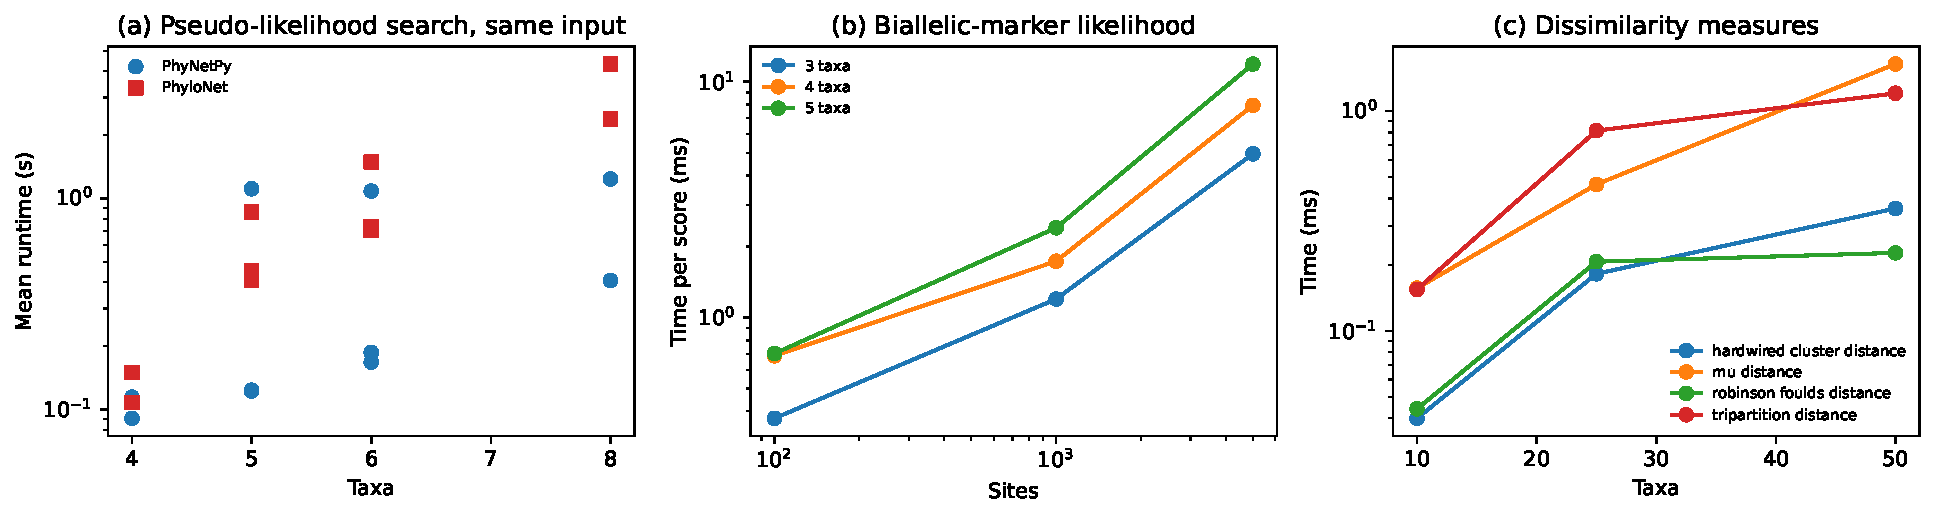
\includegraphics[width=\linewidth]{performance.pdf}
  \caption{(a) Runtime of pseudo-likelihood inference on identical input, on a
  log scale, one point per condition of Table~\ref{tab:phylonet}. Points are not
  joined because conditions sharing a taxon count differ in the number of gene
  trees. (b) Time to evaluate the exact biallelic-marker likelihood of a fixed
  network against the number of sites. (c) Dissimilarity-measure runtime against
  taxon count. Panels show runtime only; accuracy is in
  Table~\ref{tab:phylonet}. Every panel is drawn from the JSON written by the
  benchmark scripts.}
  \label{fig:performance}
\end{figure}

Gene trees were simulated under the multispecies network coalescent from a known
species tree or network, written once, and given to both implementations. Both
were asked for the same method -- pseudo-likelihood network inference, PhyloNet's
\code{InferNetwork_MPL} -- and both were given a reticulation budget equal to the
true count. The population parameter was set to $\theta = 0.5$, which leaves
between 46\% and none of the gene trees concordant with the generating topology
depending on the condition; at the simulator's smaller default scale every
simulated gene tree comes out identical to the species tree, and a comparison on
such data measures nothing. Both searches are stochastic, so each of the ten
conditions was run on three independently simulated replicates, giving 30 trials
per implementation. Table~\ref{tab:phylonet} and Figure~\ref{fig:performance}(a)
report the aggregate; per-replicate values are in the benchmark JSON.

On runtime, \phynetpy\ is faster on eight of the ten conditions, by up to about
$6\times$ at eight taxa with 200 gene trees, and the margin grows with problem
size. The two exceptions are the single-reticulation conditions at five and six
taxa, where PhyNetPy's mean runtime is the higher of the two. Because PhyloNet's
figure is self-reported and excludes JVM start-up, the comparison is conservative
in PhyloNet's favour. Both tools were run single-threaded.

The accuracy finding runs the other way, and it is the more consequential of the
two. PhyloNet recovered the generating topology exactly in 16 of 30 trials.
\phynetpy\ did so in 8 of 30 under its default settings and 7 of 30 under the
\code{phylonet} preset -- roughly half as often. The preset, which exists
precisely to match PhyloNet's per-topology parameter optimisation, does not close
the gap, and on one condition it costs several times the runtime for no
improvement. On this benchmark \phynetpy's pseudo-likelihood search is faster and
less accurate than PhyloNet's, and neither tool recovers the truth reliably on
the reticulate conditions.

We have not isolated the cause, and it would be premature to attribute it to the
search strategy. One observation argues against the simplest explanation, that
the search is merely under-run: on an eight-taxon condition it reports a log
pseudo-likelihood about two orders of magnitude worse than the score of the
generating network itself ($-9.2 \times 10^5$ against $-8.3 \times 10^3$), and
that value does not change when the iteration budget is raised from its default
to 50{,}000. More iterations would help a search that was stopping early. Two
candidate explanations remain open. Continuous parameters on the returned network
may be left un-optimised, so a near-correct topology is reported with a poor
score. And the pseudo-likelihood criterion does not enforce the branch-length
unit discipline that the full likelihood does, so a network carrying lengths on
the substitution scale is scored as though they were coalescent units. Both
are recorded as defects rather than explained away.\footnote{[TODO: resolve
before submission. Either fix the underlying cause and re-run this benchmark, or
keep this subsection as written and add the diagnosis. Do not soften the accuracy
result without new measurements.]}

Two limits on the comparison should be read with it. The simulated data come from
\phynetpy's own simulator under a model both implementations assume, which makes
the comparison reproducible from this repository and makes the runtime
measurement fair, but says nothing about robustness to model misspecification.
And while three replicates are enough to show that the accuracy difference is not
an artefact of a single lucky run, they are not enough to estimate its size
precisely; the counts in Table~\ref{tab:phylonet} should be read as indicating a
gap of roughly a factor of two rather than as a calibrated effect size.

\subsection{Component measurements}

\begin{table}[t]
  \centering
  \small
  % Generated by benchmarks/make_artifacts.py -- do not edit by hand.
\begin{tabular}{llrrrr}
\toprule
Model & Implementation & \textsc{PhyNetPy} & \texttt{expm} & Ratio & $\max|\Delta|$ \\
 & & ($\mu$s) & ($\mu$s) & & \\
\midrule
JC & closed form & 1.68 & 24.75 & 14.7$\times$ & 1.1e-16 \\
F81 & closed form & 1.32 & 24.96 & 18.9$\times$ & 1.4e-17 \\
K81 & closed form & 1.45 & 25.95 & 18.0$\times$ & 1.1e-16 \\
K80 & Tamura-Nei & 2.03 & 24.70 & 12.1$\times$ & 1.1e-16 \\
HKY & Tamura-Nei & 2.06 & 23.74 & 11.5$\times$ & 2.8e-17 \\
TN93 & Tamura-Nei & 2.04 & 24.78 & 12.1$\times$ & 1.1e-16 \\
SYM & cached eigendecomposition & 2.67 & 23.91 & 8.9$\times$ & 2.1e-16 \\
GTR & cached eigendecomposition & 2.60 & 25.45 & 9.8$\times$ & 4.4e-16 \\
\bottomrule
\end{tabular}

  \caption{Transition-matrix evaluation at $t = 0.1$ against a fresh
  \code{scipy.linalg.expm} call on the same rate matrix. Six models have a
  closed form; SYM and GTR cache an eigendecomposition. The final column is the
  largest absolute elementwise disagreement with \code{expm}, so this table is
  simultaneously a speed and a correctness measurement.}
  \label{tab:substitution}
\end{table}

\begin{table}[t]
  \centering
  \small
  % Generated by benchmarks/make_artifacts.py -- do not edit by hand.
\begin{tabular}{lrrr}
\toprule
Operation & \textsc{PhyNetPy} & NetworkX & Ratio \\
 & ($\mu$s) & ($\mu$s) & (NetworkX\,/\,\textsc{PhyNetPy}) \\
\midrule
Incident in-edges of a node & 0.16 & 1.81 & 11.45$\times$ \\
Out-degree of a node & 0.16 & 0.20 & 1.21$\times$ \\
Enumerate all leaves & 173.41 & 453.99 & 2.62$\times$ \\
Topological order & 2384.32 & 1295.26 & 0.54$\times$ \\
Leaf descendants, all nodes & 1452.37 & --- & --- \\
\midrule
Peak construction memory (KiB) & 2103 & 1111 & 0.53$\times$ \\
\bottomrule
\end{tabular}

  \caption{The compiled graph core against \code{networkx.DiGraph}
  \cite{Hagberg2008NetworkX} on the same 1{,}999-node topology. Ratios above
  one favour \phynetpy. \phynetpy\ is faster on the incidence and leaf queries
  that dominate network search and slower on topological ordering, and it uses
  roughly twice the peak memory during construction.}
  \label{tab:graphcore}
\end{table}

\begin{table}[t]
  \centering
  \small
  % Generated by benchmarks/make_artifacts.py -- do not edit by hand.
\begin{tabular}{rrrrrr}
\toprule
Taxa & Genes & Compiled (ms) & Python (ms) & Ratio & $|\Delta \log \mathrm{PL}|$ \\
\midrule
6 & 40 & 1.13 & 1.46 & 1.29$\times$ & 1.1e-13 \\
8 & 60 & 2.97 & 4.69 & 1.58$\times$ & 1.1e-12 \\
10 & 80 & 7.10 & 11.08 & 1.56$\times$ & 9.1e-13 \\
12 & 100 & 12.93 & 21.70 & 1.68$\times$ & 2.9e-11 \\
\bottomrule
\end{tabular}

  \caption{The compiled pseudo-likelihood dynamic program against the
  pure-Python reference that remains in the repository, selected by a module
  flag so that only the inner loop differs. The final column confirms the two
  paths return the same score.}
  \label{tab:kernels}
\end{table}

Three component measurements explain where \phynetpy's time goes.

Transition-matrix evaluation (Table~\ref{tab:substitution}) is between
$8.5\times$ and $19\times$ faster than calling \code{expm}, because six of the
eight models use a closed form and the remaining two cache an
eigendecomposition. This is not a claim to have improved on SciPy; it is the
expected benefit of exploiting structure that a general matrix exponential
cannot see.

The compiled graph core (Table~\ref{tab:graphcore}) is a genuinely mixed
result. Incidence lookup is about $11\times$ faster than NetworkX and
leaf enumeration about $3.8\times$, both essentially independent of network
size, which is the payoff from maintaining incidence indices. Topological
ordering is about $0.7\times$ -- that is, slower. And peak memory during
construction is roughly $1.9\times$ NetworkX's. The operations \phynetpy\
optimises are the ones a search loop performs most often, and the trade it makes
is memory for lookup speed; a reader whose workload is dominated by whole-graph
traversals rather than incidence queries should not expect a gain.

The compiled pseudo-likelihood kernel (Table~\ref{tab:kernels}) is worth
between $1.3\times$ and $1.7\times$ over the pure-Python dynamic program, with
the advantage growing with taxon count, and the two paths agree to within
$2 \times 10^{-12}$. That is a smaller factor than compiled-versus-interpreted
comparisons often report, because most of the work is already in array
operations rather than Python-level loops.

Biallelic-marker likelihood evaluation (Table~\ref{tab:snp},
Figure~\ref{fig:performance}(b)) takes about $1.1$\,ms for three taxa and
1{,}000 sites, scaling roughly linearly in sites and more steeply in taxa, as
the exact algorithm's dependence on the number of sampled lineages implies. The
first evaluation in a process costs noticeably more than subsequent ones
because the likelihood model is constructed on first use; both figures are
recorded, since a single interactive score and a score inside a search loop are
different quantities.

\begin{table}[t]
  \centering
  \small
  % Generated by benchmarks/make_artifacts.py -- do not edit by hand.
\begin{tabular}{rrrr}
\toprule
Taxa & Sites & Time per score (ms) & $\log L$ \\
\midrule
3 & 100 & 0.37 & -106.2 \\
3 & 1000 & 1.20 & -1030.6 \\
3 & 5000 & 4.94 & -5161.8 \\
4 & 100 & 0.69 & -114.2 \\
4 & 1000 & 1.73 & -1067.0 \\
4 & 5000 & 7.94 & -5774.7 \\
5 & 100 & 0.70 & -120.9 \\
5 & 1000 & 2.40 & -1196.6 \\
5 & 5000 & 11.89 & -6461.3 \\
\bottomrule
\end{tabular}

  \caption{Exact biallelic-marker likelihood of a fixed network, median of
  repeated evaluations with the likelihood model already constructed. The
  single-evaluation cost, which includes that construction, is recorded
  alongside these figures in \code{benchmarks/snp.json}.}
  \label{tab:snp}
\end{table}

\subsection{What is not measured}

Three gaps should be read alongside the tables above. No comparison against
PhyloNet's Bayesian samplers is reported: matching two MCMC implementations
requires agreeing on chain length, proposal weights and convergence criteria
before any timing is meaningful, and that comparison has not been done.
No empirical dataset is analysed here. And every measurement comes from one
machine, so the ratios should be read as indicative rather than as portable
constants.

\section{Moving from PhyloNet to \phynetpy}
\label{sec:comparison}

This section is addressed to researchers with working PhyloNet analyses. The
useful question is not which tool is better but what specifically changes, and
what does not carry over.

\begin{figure}[t]
  \centering
  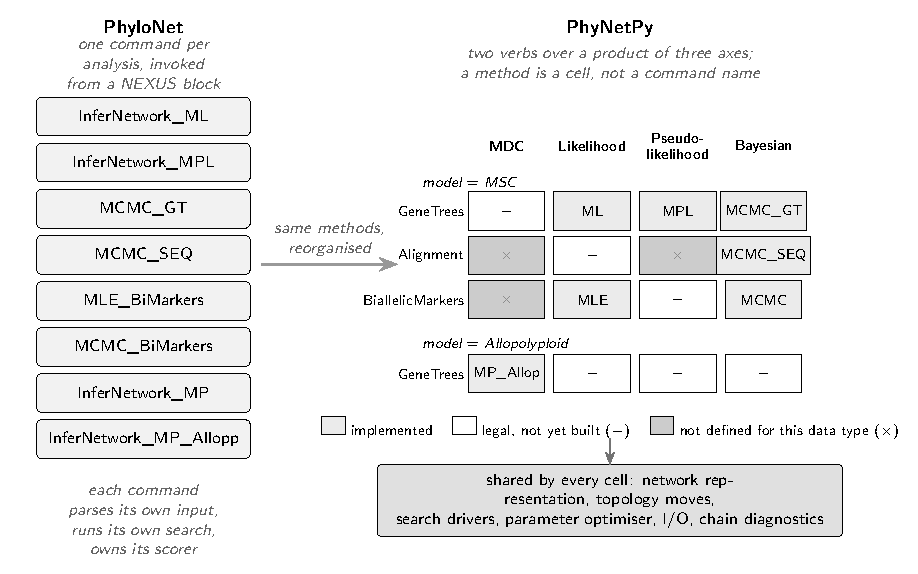
\includegraphics[width=\linewidth]{transition.pdf}
  \caption{The same body of methods under two organisations. On the left each
  analysis is a named command that handles its own input, search and scoring.
  On the right the analyses are cells of a product of three axes over shared
  machinery, so the empty cells are visible and distinguishable: $-$ marks a
  combination that is well defined but unbuilt, $\times$ one that is not
  defined for that data type. The figure makes no claim that one organisation
  produces better inferences.}
  \label{fig:transition}
\end{figure}

\begin{table}[t]
  \centering
  \scriptsize
  % Comparison of PhyloNet and PhyNetPy.
%
% Hand-written, unlike the numeric tables, because the rows are qualitative.
% Every PhyNetPy entry is verified against the 0.6.0 source; see INVENTORY.md.
% PhyloNet entries describe version 3.8.2 as distributed and are drawn from its
% published description and its command set.
%
% Rows marked [TODO] could not be verified from the material available and must
% be checked against PhyloNet's documentation before submission.

\begin{tabular}{@{}p{38mm}p{52mm}p{52mm}@{}}
\toprule
& \textbf{PhyloNet 3.8.2} & \textbf{\textsc{PhyNetPy} 1.0.0} \\
\midrule

Implementation language
& Java
& Python, with four Cython extension modules \\

Invocation
& A NEXUS file containing a \texttt{PHYLONET} block, run through
  \texttt{java -jar}
& Python function calls; no driver file \\

Programmatic API
& Java classes are reachable by writing Java against the jar
& The documented surface is the package itself: 121 exported names, two
  inference verbs plus \texttt{simulate} \\

Analysis organisation
& One named command per analysis
& A method is a (data, model, criterion) cell; dispatch goes through a
  registry that also reports validity \\

Adding a method
& Implement a new command
& Register one cell with \texttt{@register}; search drivers, moves,
  parameter optimiser and I/O are inherited \\

Network representation
& Internal to the tool
& \texttt{Network}: a reusable rooted DAG, independent of any analysis, with
  no cap on reticulation in-degree \\

Distinguishing invalid from unbuilt requests
& An unsupported combination surfaces as a command-level error
& \texttt{TypeError}, \texttt{ValueError} and \texttt{NotImplementedError} are
  raised for three distinct causes \\

\midrule
\multicolumn{3}{@{}l}{\emph{Analyses}} \\

Maximum likelihood from gene trees
& \texttt{InferNetwork\_ML}
& Available \\

Maximum pseudo-likelihood from gene trees
& \texttt{InferNetwork\_MPL}
& Available \\

Bayesian from gene trees
& \texttt{MCMC\_GT}
& Available \\

Bayesian from sequences
& \texttt{MCMC\_SEQ}
& Available \\

Marker likelihood
& \texttt{MLE\_BiMarkers}
& Scoring available; the search path raises \\

Bayesian from markers
& \texttt{MCMC\_BiMarkers}
& Available \\

Maximum parsimony, diploid hybridization
& \texttt{InferNetwork\_MP}
& Not in 0.6.0; scheduled for 1.0.0 \\

Maximum parsimony under polyploidy
& \texttt{InferNetwork\_MP\_Allopp}
& Available, with bootstrapping \\

\midrule
\multicolumn{3}{@{}l}{\emph{Supporting capability}} \\

Simulation
& Available as separate commands
& \texttt{simulate} inverts the same axes and returns a data object that feeds
  \texttt{infer} directly; gene trees, sequences and markers under
  \texttt{MSC} only \\

Network comparison
& Distance commands are provided
& Nine dissimilarity measures plus a reticulation-specific comparison module
  (tripartitions, precision and recall) \\

Chain diagnostics
& Output is written for external tools
& ESS, autocorrelation time, HPD intervals, Geweke and Gelman--Rubin
  in-process; Tracer and NEXUS output for external tools \\

Visualisation
& \textbf{[TODO: verify what PhyloNet 3.8.2 provides]}
& ASCII rendering only \\

Across-site rate heterogeneity
& \textbf{[TODO: verify]}
& Not implemented \\

\midrule
\multicolumn{3}{@{}l}{\emph{Distribution and testing}} \\

Installation
& Download a jar; requires a JVM
& \texttt{pip install phynetpy}; requires a C compiler when building from
  source \\

Automated testing
& \textbf{[TODO: verify what PhyloNet publishes]}
& 1{,}130 tests, 1{,}125 passing in the default run \\

Continuous integration
& \textbf{[TODO: verify]}
& GitHub Actions across Python 3.9--3.14, plus Windows and packaging jobs \\

Numerical cross-validation
& ---
& 14 cases checked against PhyloNet itself to a tolerance of $10^{-5}$ \\

License
& \textbf{[TODO: verify PhyloNet's license]}
& MIT \\

\bottomrule
\end{tabular}

  \caption{PhyloNet 3.8.2 and \phynetpy\ 1.0.0. \phynetpy\ entries are verified
  against the source; entries marked \textbf{[TODO]} could not be established
  from the material available and must be checked against PhyloNet's
  documentation before submission rather than guessed.}
  \label{tab:comparison}
\end{table}

\subsection{What changes}

\paragraph{The driver file disappears.}
A PhyloNet analysis is a NEXUS file with a \code{PHYLONET} block, executed
through \code{java -jar}. Parameters are positional and flag-based inside that
block, and a sweep over conditions means generating files. In \phynetpy\ the
analysis is Python: a loop over $\theta$ values or reticulation budgets is a
loop, and intermediate results stay as objects.

\paragraph{Choosing a method becomes choosing arguments.}
Switching from maximum likelihood to pseudo-likelihood changes one argument
rather than one command name, and the return type does not change with it. In
PhyloNet the corresponding change is to a different command with its own syntax
and output format.

\paragraph{Results are objects, not text to parse.}
PhyloNet writes inferred networks and scores to standard output, and a pipeline
around it is usually a parser. \code{infer} returns an \code{InferenceResult}
whose \code{.best} is a \code{Network} that the distance functions, the
decomposition routines and \code{score} all accept directly. This is the
practical difference most PhyloNet users will notice first.

\paragraph{Unsupported requests say which kind of unsupported they are.}
The three-way distinction between \code{TypeError}, \code{ValueError} and
\code{NotImplementedError} tells a user whether to change the data, change the
criterion, or wait.

\subsection{What does not carry over}

\paragraph{Input files are not automatically compatible.}
\phynetpy\ reads extended Newick, NEXUS, FASTA and VCF, so the \emph{data} in a
PhyloNet NEXUS file is usually readable. The \code{PHYLONET} command block is
not: there is no translator from a PhyloNet block to a \phynetpy\ call, and the
migration is a rewrite of the driver, not a conversion.

\paragraph{Results will not be identical.}
The two implementations agree on the likelihood of a fixed network to $10^{-5}$
(Section~\ref{sec:validation}), but searches are stochastic and their proposal
kernels differ, so inferred networks can differ --- and in
Section~\ref{sec:headtohead} they did on one reticulate condition. The
\code{phylonet} search preset exists to narrow this gap when the point is a
comparison rather than an analysis, by reproducing PhyloNet's
optimise-every-parameter-per-topology behaviour.

\paragraph{Some analyses are not available.}
Maximum parsimony from gene trees under diploid hybridization is absent, and
marker maximum likelihood can score but not search. Anyone whose work depends on
those should continue to use PhyloNet.

\paragraph{Installation requirements differ.}
PhyloNet needs a JVM and a jar. \phynetpy\ installs with \code{pip}, but the
compiled graph core is required, so installing from a source distribution needs
a C compiler. Where a wheel is published for the target platform this does not
arise.

\subsection{A worked correspondence}

A PhyloNet pseudo-likelihood analysis reads, inside a NEXUS file:

\begin{lstlisting}[language={}]
BEGIN PHYLONET;
InferNetwork_MPL (gt1,gt2,...,gt100) 1 -pl 4;
END;
\end{lstlisting}

The corresponding \phynetpy\ analysis:

\begin{lstlisting}
from phynetpy.data import GeneTrees
from phynetpy.criteria import PseudoLikelihood
from phynetpy.infer import infer

gts = GeneTrees.from_file("genes.nex", {"A": ["A1", "A2"], "B": ["B1"]})
result = infer(gts, criterion=PseudoLikelihood(), max_reticulations=1)
\end{lstlisting}

The species-to-allele mapping moves from a \code{-a} flag into the data object,
where it travels with the data it describes instead of being restated per
command. The reticulation budget is a keyword rather than a positional integer.
The gene trees are named once, by file, rather than enumerated in the call.

These two are not equivalent in every respect, and the differences are the
point of this section rather than a caveat to it: the searches differ, the
defaults differ, and \code{-pl 4} requests four-way parallelism from PhyloNet
whereas the \phynetpy\ call above is single-threaded. A migration should
re-establish results on data with a known answer rather than assume the two
calls are interchangeable.

\section{Example workflows}
\label{sec:examples}

Every listing below is an excerpt of a function in
\code{paper/phynetpy-1.0.0/listings/paper_listings.py}, which runs as a script
and fails loudly if any listing stops matching the API. Figure~\ref{fig:workflow}
shows how the pieces fit together.

\begin{figure}[t]
  \centering
  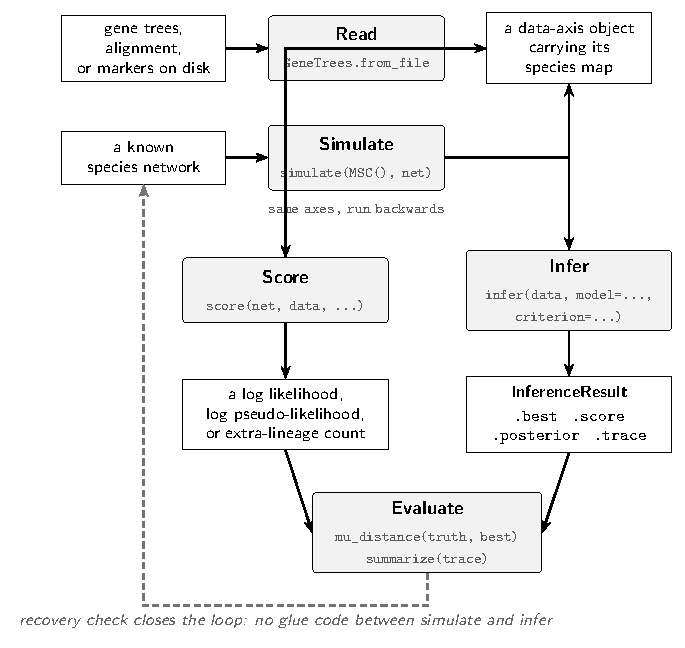
\includegraphics[width=0.78\linewidth]{workflow.pdf}
  \caption{A simulate--infer--evaluate loop in the public API. Data enters
  either by reading a file or by simulating from a known network; the two verbs
  act on it; the evaluation step closes the loop. Because \code{simulate}
  returns the same kind of object that \code{infer} consumes, a recovery check
  needs no intermediate conversion.}
  \label{fig:workflow}
\end{figure}

\subsection{Building and inspecting a network}

Reticulations are written in extended Newick and the resulting object supports
the structural queries directly.

\begin{lstlisting}
from phynetpy import blobs, count_reticulations, level, read_newick

net = read_newick("((A:0.1,(B:0.2)#H1:0.1):0.3,(#H1:0.2,C:0.3):0.2);")

count_reticulations(net)   # 1
level(net)                 # 1
net.is_acyclic()           # True
len(blobs(net))            # 4
\end{lstlisting}

The same type can be assembled node by node, which is what a method that
proposes topologies does internally:

\begin{lstlisting}
from phynetpy import Edge, Network, Node

root, internal = Node("Root"), Node("I1")
a, b, c = Node("A"), Node("B"), Node("C")
net = Network()
net.add_nodes([root, internal, a, b, c])
for edge in (Edge(root, internal), Edge(root, c),
             Edge(internal, a), Edge(internal, b)):
    net.add_edges(edge)
\end{lstlisting}

\subsection{Scoring a network, then inferring one}

This listing shows the unit discipline in use. The simulator writes branch
lengths in expected substitutions per site; the gene-tree criteria read
coalescent units. Converting is a call, not an assumption.

\begin{lstlisting}
from phynetpy import BranchLengthUnit, convert_network_branch_lengths
from phynetpy.criteria import Likelihood, PseudoLikelihood
from phynetpy.infer import infer, score, simulate
from phynetpy.models import MSC

theta = 0.5
gts = simulate(MSC(theta=theta), taxa=6, n=200, data="gene_trees", seed=3)
truth = convert_network_branch_lengths(
    gts.true_network, BranchLengthUnit.COALESCENT_2N, theta=theta
)

score(truth, gts, model=MSC(theta=theta), criterion=Likelihood())
#  -514.956
score(truth, gts, model=MSC(theta=theta), criterion=PseudoLikelihood())
# -1883.194

result = infer(gts, criterion=PseudoLikelihood(), max_reticulations=0)
result.method        # 'InferNetwork_MPL'
result.score         # -1882.494
\end{lstlisting}

Changing \code{criterion} to \code{Bayesian()} turns the same call into a
posterior sample, and \code{result.posterior} is then populated. The rest of the
call, and the type it returns, do not change.

\subsection{Simulation and recovery}

Because \code{simulate} produces a data-axis object, a recovery check is two
lines. This is the pattern behind the benchmark in
Section~\ref{sec:headtohead} and behind \code{Examples/sim_recovery.py}.

\begin{lstlisting}
from phynetpy.GraphUtils import mu_distance
from phynetpy.infer import infer, simulate

sim = simulate(MSC(theta=0.5), taxa=6, n=200, data="gene_trees", seed=11)
recovered = infer(sim, criterion=PseudoLikelihood(), max_reticulations=0)

mu_distance(sim.true_network, recovered.best)   # 0
\end{lstlisting}

The generating network is attached to the simulated data as
\code{.true_network}, so the comparison does not require tracking it separately.

\subsection{Inspecting and extending the method set}

The set of available methods is queryable rather than documented separately:

\begin{lstlisting}
from phynetpy.infer import validity_matrix

for data, row in validity_matrix().items():
    print(data, row)
\end{lstlisting}

\begin{lstlisting}[language={}, basicstyle=\ttfamily\scriptsize]
GeneTrees        {'MDC': '-', 'Likelihood': 'InferNetwork_ML',
                  'PseudoLikelihood': 'InferNetwork_MPL', 'Bayesian': 'MCMC_GT'}
Alignment        {'MDC': 'x', 'Likelihood': '-',
                  'PseudoLikelihood': 'x', 'Bayesian': 'MCMC_SEQ'}
BiallelicMarkers {'MDC': 'x', 'Likelihood': 'MLE_BiMarkers',
                  'PseudoLikelihood': '-', 'Bayesian': 'MCMC_BiMarkers'}
\end{lstlisting}

Adding a criterion means declaring what it accepts and registering an engine for
it. The objective below is deliberately trivial -- total branch length -- so that
the mechanism rather than the statistics is visible:

\begin{lstlisting}
from phynetpy.criteria import Criterion
from phynetpy.data import GeneTrees
from phynetpy.infer import Engine, register, score
from phynetpy.models import MSC

class TreeLength(Criterion):
    accepts_data = (GeneTrees,)
    scorable = True
    use_branch_lengths = False

@register(GeneTrees, MSC, TreeLength)
class TreeLengthEngine(Engine):
    method = "TreeLength"

    def infer(self, data):
        raise NotImplementedError("scoring only")

    def score(self, network, data, optimize=False):
        return sum(e.get_length() or 0.0 for e in network.E())
\end{lstlisting}

After that, \code{score(net, data, criterion=TreeLength())} dispatches to the new
engine, \code{validity_matrix()} shows the new column, and an unregistered
combination involving \code{TreeLength} raises \code{NotImplementedError} rather
than silently falling back. A real criterion would additionally implement
\code{infer}, and would get the search drivers, topology moves and parameter
optimiser from the shared layer rather than reimplementing them.

\section{Discussion}
\label{sec:discussion}

\subsection{Infrastructure as the contribution}

The methods in Table~\ref{tab:analyses} are mostly not new. What is new is that
they sit on shared components: one network type, one set of topology moves, one
parameter optimiser, one I/O layer, one set of chain diagnostics. A developer
adding a criterion writes the criterion.

Whether this lowers the barrier enough to change how network methods get built is
not something this paper can settle. The registry is exercised by seven methods,
all of them ours, and an interface that suffices for its author is weaker
evidence than one an outside contributor found sufficient. The design argument is
stated in Section~\ref{sec:architecture}; the measurement that would test it does
not exist yet.

Two design decisions seem worth keeping regardless. Making the validity of a
(data, model, criterion) triple a runtime query, rather than prose in
documentation, means the method set cannot drift from its description --
Table~\ref{tab:analyses} is generated from the registry. And separating the three
failure modes gives a user an actionable answer: change the data, wait for a
release, or reconsider the question.

\subsection{What the Python implementation does and does not buy}

Being a Python library makes some things straightforward that were awkward
before. An inferred network is an object that goes directly into a distance
function, a plotting call, or a pandas frame. A sweep over reticulation counts is
a loop. Simulation and inference compose without an intermediate file, which is
what makes the recovery check in Section~\ref{sec:examples} two lines.

It does not, by itself, make anything faster. \phynetpy's runtime advantage in
Section~\ref{sec:headtohead} comes from compiled kernels and from algorithmic
choices such as incremental rescoring, not from the choice of language -- and the
component measurements show the trade is not uniform: the graph core is faster on
incidence queries and slower on whole-graph traversal, using about twice the
memory. Claims that one language is faster than another are not what this section
is for.

Integration with the numerical and machine-learning ecosystem is often cited as a
reason to work in Python, and the architecture does make it practical: the
network is an ordinary object, likelihoods are ordinary callables, and a scorer
backed by PyTorch or JAX could be registered as a cell without changing anything
else. \phynetpy\ 1.0.0 contains no machine-learning functionality, no
differentiable likelihood and no GPU support beyond an optional CuPy path in the
marker likelihood. The integration is available rather than done.

\subsection{Reproducibility}

Two properties of the release matter for reproducing results. The version is
single-sourced and CI verifies that a clean install of both the wheel and the
source distribution reports it, so a paper citing a version is citing something
checkable. And the parts of an analysis that affect results -- the model
parameters, the criterion, the search preset, the seed -- are arguments at the
call site rather than defaults buried in a driver file.

The benchmark scripts for this paper follow the same discipline: each writes a
JSON file recording package versions, interpreter, platform, replicate counts and
seeds, and the tables and figures are generated from those files. This is why the
accuracy result in Section~\ref{sec:headtohead} is reported as it is. It emerged
from re-running a benchmark rather than from reading code, and a pipeline that
only regenerated favourable numbers would not have surfaced it.

\subsection{Limitations}

Relative to PhyloNet, \phynetpy\ 1.0.0 lacks maximum parsimony from gene trees
under diploid hybridization, and its marker maximum likelihood can score a
network but not search. Both are visible in \code{validity_matrix()}.

The accuracy deficit in Section~\ref{sec:headtohead} is the most consequential
open item. Across 30 trials of matched pseudo-likelihood inference PhyloNet
recovered the generating topology 16 times and \phynetpy\ 8, and the
\code{phylonet} preset intended to make the comparison like-for-like did not
close the gap. Anyone whose work depends on pseudo-likelihood network inference
should validate against PhyloNet on data with a known answer before relying on
\phynetpy\ for it.

Other limits are narrower. Across-site rate heterogeneity is not implemented, so
sequence analyses cannot fit a discretised gamma over sites. Simulation supports
only the \code{MSC} model; the allopolyploid model has no simulator. The network
simulator grafts reticulations onto a separately drawn tree rather than running a
birth--death--hybridization process, so it should not be used to study the
distribution of network shapes. Visualisation is ASCII text. There is no network
classifier for the graph-theoretic classes beyond level, and no summarisation of
\emph{sets} of networks, which is what a Bayesian run most wants. One compiled
kernel, \code{seq_engine_cy}, is built but not yet called. Installing from source
needs a C compiler. And every measurement in this paper comes from one machine.

\subsection{Future work}

The immediate items are the two unbuilt cells and a diagnosis of the accuracy
result. Beyond those: connecting the compiled sequence kernel; rate
heterogeneity; a birth--death--hybridization simulator; network classification
and set-level summarisation; and visualisation, where writing Tracer and NEXUS
output has so far been a substitute for having any of our own.

The architecture suggests directions we have not taken. A differentiable
pseudo-likelihood would make gradient-based optimisation over continuous
parameters available; a learned proposal distribution would fit the
\code{ProposalKernel} interface; approximate Bayesian computation would compose
with \code{simulate} directly. These are plausible because the pieces are
separable, not because any of them is underway.

\section{Conclusions}
\label{sec:conclusion}

\phynetpy\ 1.0.0 provides a Python foundation for phylogenetic network work:
a reusable network type, an analysis layer that does not depend on any inference
method, and seven inference methods reached through two verbs over three typed
axes. Six of those methods correspond to PhyloNet analyses, and the
likelihood functions underlying two of them agree with PhyloNet's own to
$10^{-5}$ across fourteen adversarial cases.

It is a successor to PhyloNet in the sense that it continues the same line of
software and reimplements much of the same body of methods. It is not a
replacement. Two PhyloNet analyses have no counterpart here, PhyloNet command
files do not carry over, and on the one search we compared directly PhyloNet
recovered the true topology about twice as often as we did. Where those matter,
PhyloNet remains the right tool.

The case for building on \phynetpy\ is about what the next method costs. A new
criterion is a class and a registry entry, and it inherits the network
representation, the topology moves, the parameter optimiser and the diagnostics
rather than restating them.

\section{Reproducibility and software citation}
\label{sec:reproducibility}

\subsection{Reproducing the results in this paper}

Every number, table and figure in Sections~\ref{sec:validation}
and~\ref{sec:examples} is produced by scripts in
\code{paper/phynetpy-1.0.0/}. Running

\begin{lstlisting}[language=bash, basicstyle=\ttfamily\small]
export PHYLONET_JAR=/path/to/phylonet.jar
python paper/phynetpy-1.0.0/benchmarks/run_all.py
python paper/phynetpy-1.0.0/benchmarks/make_analyses_table.py
python paper/phynetpy-1.0.0/listings/paper_listings.py
\end{lstlisting}

regenerates the benchmark JSON, rewrites \code{tables/*.tex} and
\code{figures/performance.pdf} from it, rebuilds Table~\ref{tab:analyses} from
the live dispatch registry, and executes every code listing. The PhyloNet
comparison is skipped with a warning if no jar is configured; the rest needs
nothing beyond the package and its dependencies. The tables under
\code{tables/} are generated files and carry a header saying so.

\subsection{Environment}

Measurements in this paper were taken under the following configuration, which
each benchmark script also records in the \code{meta} block of its own JSON
output:

\begin{itemize}
  \item \phynetpy\ 0.6.0.\footnote{[TODO: re-run every benchmark against the
    tagged 1.0.0 release and update this section, the abstract and
    Section~\ref{sec:validation}. The measurements reported here were taken on
    the 0.6.0 codebase, which is 1.0.0 without the two unbuilt cells of
    Table~\ref{tab:analyses}.]}
  \item CPython 3.14.2 on Windows 11 (build 10.0.26200), AMD64.
  \item AMD Family 25 Model 97 (Zen 4 class), single-threaded unless stated.
  \item NumPy 2.3.5, SciPy 1.16.3, NetworkX 3.6.1.
  \item PhyloNet 3.8.2 (\code{phylonet.jar}, 41{,}019{,}851 bytes) under
    Java 1.8.0\_491, with BEAGLE for the Felsenstein cross-check.
\end{itemize}

Random seeds are fixed in every script and recorded per measurement. The
head-to-head comparison runs three replicates per condition, replicate $i$ using
seed $20260925 + i$ for both simulation and \phynetpy's search; the component
benchmarks use seeds 7 and 11, and the marker timings use seed 1. PhyloNet's
search is stochastic and its command-line interface is not seeded here, so its
variation across replicates is uncontrolled -- which is part of why the
comparison is replicated rather than run once. The generating network for each
replicate is stored as Newick in the benchmark JSON alongside its results,
together with the gene-tree concordance that replicate produced, so any trial can
be reconstructed exactly.

\paragraph{Timing protocol.} Microbenchmarks report the median of repeated
batches measured with \code{time.perf_counter}, after one warm-up call; loop and
repeat counts are stored per measurement. Interpreter start-up and module import
are excluded and recorded separately. For the PhyloNet comparison, PhyloNet's
self-reported running time is used because it excludes JVM start-up and is
therefore comparable to \phynetpy's in-process timing; total wall time including
JVM start-up is also recorded in the JSON. No result in this paper uses
multi-threading or GPU offload.

\paragraph{Datasets.} All data are simulated by \phynetpy\ itself, from seeds
recorded in the scripts, so no external archive is required. No empirical dataset
is analysed in this paper.

\subsection{Citing \phynetpy}

\begin{itemize}
  \item Software: \phynetpy\ version 1.0.0.
  \item Repository: \url{https://github.com/NakhlehLab/PhyNetPy}, tag
    \code{v1.0.0}.\footnote{[TODO: create the \code{v1.0.0} tag and confirm this
    reference before submission; the current release tag is \code{v0.6.0}.]}
  \item Package: \url{https://pypi.org/project/phynetpy/}.
  \item License: MIT.
  \item Archived release: \cite{TODO_PhyNetPy_archive}.
\end{itemize}

Methods reimplemented from published work should be cited to their original
sources rather than to \phynetpy\ or to PhyloNet generically; the relevant
citation for each is given in Table~\ref{tab:analyses}.


\section*{Acknowledgements}

This work was supported by the National Science Foundation under award
IIBR 2420499. % [TODO: confirm the award acknowledgement wording required by NSF]

\bibliographystyle{unsrtnat}
\bibliography{references}

\end{document}
